% !TeX root = ../main.tex
\chapter{Broadband photon pair generation}

Back to the classical nonlinear optics theory, the solution to nonlinear coupling equations requires the initial power at ether signal or idler mode, which is called seed in the laser terminology. However, in quantum classical theory, all the modes in cavity behave intrinsic vacuum fluctuation at the quantity of half $ \hbar \omega $. Thus, even without light fed, the quantum fluctuation leads to enhancement at the single photon levels. The intracavity pump power then behaves the amplifier, intensify the corresponding signal or idler mode photon flux. Once the single photon flux exceeds cavity threshold, the extracavity single photon can be detected. To note, these kind of excitation is indistinguishable because the signal and idler photons are emitted simultaneously as a result of quantum mechanics, rather than signal photon stimulates idler photon and vice versa. In the context of quantum states, the state created intracavity is at the superposition of signal state and idler state. The wave packet is different from the normal single photon one. Further theoretical research \cite{Scully1997} explained the squeezed nature of four wave mixing photon pairs, which is one of the exclusive properties of frequency entangled photon pair.

In general, the spontaneous four wave mixing in nonlinear cavities defined in our context refers to the cavity modes are excited collectively and pair-by-pair under the phase matching condition. Thus, under the weak coherent approximation, the photon pair only include one photon in each mode but correlated with each other. Thus, the conventional coincidence counting technology can be used to verify such correlation. In the term of generation band, it agrees with the classical phase matching condition at pump power limit.

%Furthermore, 
%To clarify with the physics compared with the relevant research, such as Kerr frequency comb and soliton generation, where ultra-high power is used to built intracavity pump mode, the spontaneous four wave mixing differs 
%\cite{Chembo2016a}

\section{Methods}

Using the dispersion extraction method in previous chapter, zero dispersion wavelength can be located easily among the measured band. Optical telecom band is focused on in this research due to enormous available fiber optical components for totally in-line setups. 
Illustrated in \autoref{fig:bibpf}, the setup of mode-resolvable singular photon pair generation adopts the tunable laser as the pump power whose display tunability is 0.1 pm. The laser output is first connected to ring resonators using the same fiber launching system and measured with the power meter. A simple transmission scanning is perform to select the built-in polarization. For the high \textit{Q}-factor devices, the transmission of TE and TM modes are separated in a distance of tens of pm. Thus, as either of the resonance vanished, the input polarization is aligned at particular mode. For low \textit{Q}-factor cavities, the method of polarization alignment is as same as the one used in spectra transmission scanning.

Next, the output light are splitted 50\si{\percent}:50\si{\percent}, indicating half of photons are lost, and sequentially filtered through two sets of band pass filters. The 3dB bandwidths of first set are 1540$\pm$4 nm and 1560 $\pm$4 nm, respectively. The second ones are tunable and 0.12nm-wide. Since the mode spacing is 0.75 nm for 100GHz-FSR cavities, the tunable band pass filter is adequate to define the single mode. Finally, each channel are detected using superconducting single photon detectors (SNSPD) in the resolution of 100 ps. Since the SNSPD is polarization-sensitive, another two polarization controllers (not shown) are used to achieve highest single photon counting. The time controller (ID900, ID Quantique) collects and records the count signal to calculate the coincidence counts.

\begin{figure}
	\centering
	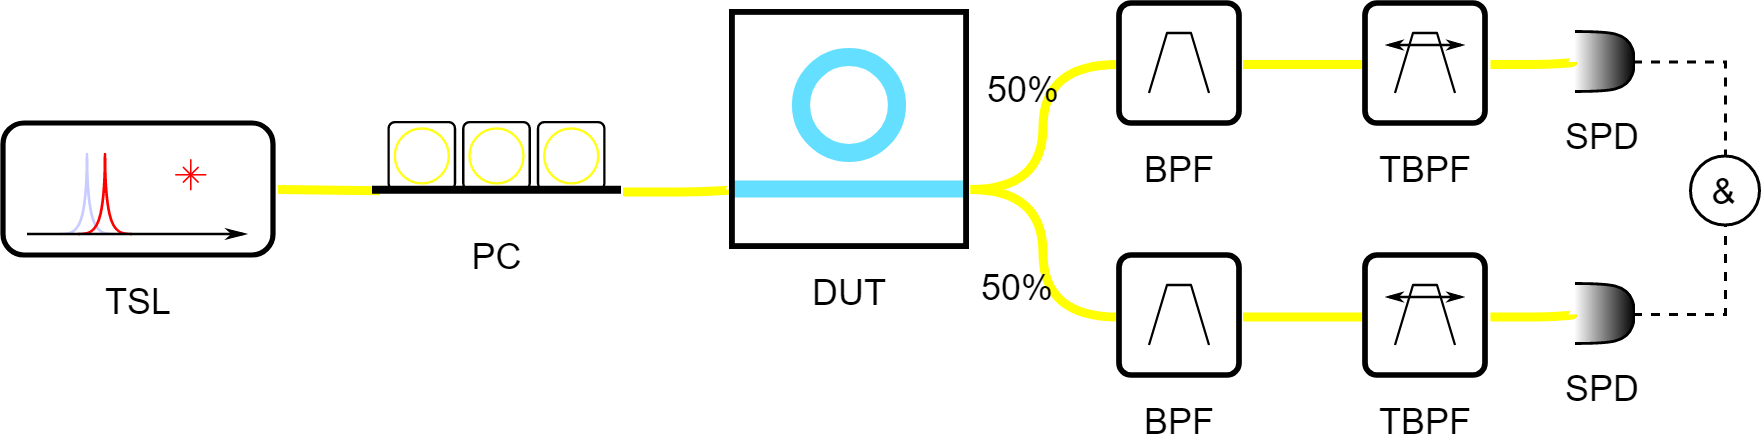
\includegraphics[width=0.9\linewidth]{imgs/png/biBPF}
	\caption{Mode-resolvable singular photon pair generation}
	\label{fig:bibpf}
\end{figure}

\bigskip
\noindent\textbf{Coincidence counting}

In quantum optics, coincidence counting is usually used to examine the non-locality of singular wave-particle. In our case, the photons splitted into two channels A and B, yields the count per second $N_A$ and $ N_B $. Define the coincidence windows $t$ 1 ns commonly, and coincidence count (CC) is two photon trigger events within this time window, equivalent to the photon pair generation rate effectively. The accidental counting (ACC) is defined as $ N_A N_B t $. To reduce the noise effect, accidental-coincidence ratio (CAR) is defined as CC/ACC.


It is worth to mention that in our research, the main topic is generation rather than manipulation, in result numerous band-pass filters are exploited to realize mode-resolvable single photon counting. It does not contradict with distinguishability nature of frequency correlated photon pairs.


\section{Photon flux}

With the pump power set as -10 dBm, 100 \si{\micro\watt} and central wavelength at 1550.64 nm, the result of photon flux versus relative mode index is presented in \autoref{fig:flux1}. The device selected is 150 GHz FSR and shows anomalous dispersion at 1550 nm. The relative mode index is collect from 7-14, since the bandwidth of BPFs is 8 nm, around 7 times of FSR. To achieve higher photon counting, the central wavelength of TBPF is tuned carefully.

There is tendency that photo flux is decreasing as the mode index increases. It can be explained that phase mismatch at farther mode pair is greater. The difference between signal and idler bands origins from the asymmetry at phase matching condition. 
%However, the problematic factor during our measurement is that all the data are collected after several BPFs.  But due to the backlash of mechanical unit

\begin{figure}
	\centering
	\includesvg[width=3in]{photon/flux_1}
	\mycaption{Photon flux at 100 \si{\micro\watt} of Ligentec group 2 device 1}{}
	\label{fig:flux1}
\end{figure}




\section{Pump power dependence}

